\chapter{Cónicas}

\begin{tikzpicture}
	\fill [left color=red!50, right color=teal!50] (0,0) rectangle (6.5,.2);
	\fill [left color=teal!50, right color=blue!50] (6.5,0) rectangle (11.5,.2);
	\end{tikzpicture}

\vspace{5mm}


\begin{adjustwidth}{40pt}{40pt}
\begin{cuadro-gris}

	\begin{multicols}{2}
	$\triangleright \quad$  Cónicas: circunferencia, parábola, elipse e hipérbola.
	
	$\triangleright \quad$  Desplazamiento de las cónicas.
	
	$\triangleright \quad$  Excentricidad de las cónicas.
	
	$\triangleright \quad$  Propiedades de reflexión de las cónicas.
	\end{multicols}
	
\end{cuadro-gris}
\end{adjustwidth}


\vspace{5mm}
La primera definición conocida de sección cónica surge en la Antigua Grecia, cerca del año 340 a. C., (Menecmo) donde fueron definidas como secciones ``de un cono circular recto''. Los nombres de \emph{parábola(1), elipse(2) e hipérbola(3)} se deben a Apolonio de Perge (Perge, c. 262 a, C, - Alejandría, c. 190 a. C.), conocido con el sobrenombre de El Gran Geómetra.  Aunque en la época en que se estudiaron no había posibilidad de ver su aplicabilidad en la ciencia, su importancia quedó justificada con el paso del tiempo. \textcolor{gris}{Si el plano que corta al cono lo hace perpendicularmente a su eje de simetría se obtiene la \emph{circunferencia}.}

\begin{figure}[H]
	\centering
	\includegraphics[width=.7\textwidth]{img-conicas/conicas00.png}
	\end{figure}

Las cónicas se pueden estudiar de varias formas:

\begin{itemize}
\item Como lo hicieron los griegos, como la intersección de un plano con dos conos invertidos y unidos por el vértice.
\item Como casos particulares la las formas cuadráticas: $\ Ax^2+By^2+Cxy+Dx+Ey+F=0$
\item Como \emph{lugares geométricos} de puntos del plano que cumplen una determinada condición. Esta es la forma en que veremos las cónicas.
\end{itemize}

%%%%%%%%%%%%%%%%%%%%%%%%%%%%%%%%%%%%%%%%%%%%%%%%%%
\vspace{5mm}
\section{Elipses}
\vspace{-5mm}

\begin{tikzpicture}
	\fill [left color=red!50, right color=teal!50] (0,0) rectangle (3.5,.1);
	\fill [left color=teal!50, right color=blue!50] (3.5,0) rectangle (7.5,.1);
	\end{tikzpicture}
\vspace{0.5cm}

\begin{definition}[ Elipse]

\textbf{\emph{Elipse}:} conjunto de los puntos del plano cuya \underline{suma} de distancias a dos puntos fijos llamados \emph{focos}, $\boldsymbol F\ \text{ y } \boldsymbol{F'}$, es un valor constante $\boldsymbol{2a}$.	
\end{definition}


\vspace{4mm}
\begin{multicols}{2}
\underline{Elementos de la elipse}:
\begin{figure}[H]
	\centering
	\includegraphics[width=.5\textwidth]{img-conicas/conicas06.png}
	\end{figure}	
	\begin{itemize}
	\item La recta que pasa por los focos es el \emph{eje focal}.
	 

	\item El punto medio entre los focos es el \emph{centro} $C$ de la elipse.

	\item Las intersecciones de la elipse con el eje focal son los \emph{vértices}, $V$ y $V'$. 

	\item La distancia entre los vértices, $2a$, es el \emph{eje mayor} de la elipse.
	\end{itemize}
\end{multicols}

\vspace{4mm}

Caso sencillo: focos en $\mathcal OX$, $\ F(c,0);\ \ F'(-c,0)\, . \ $ Por definición, $\ d(P,F)+d(P,F')=2a$, luego

$\sqrt{(x-c)^2+y^2}+\sqrt{(x+c)^2+y=2}=2a \ \to \ (\sqrt{(x+c)^2+y^2})^2=(2a-\sqrt{(x-c)^2+y^2})^2$

$(x+c)^2 + \cancel{y^2} = 4a^2 + (x-c)^2 +\cancel{y^2} -4a\sqrt{(x-c)^2+y^2} \ \to \ $

$\to \ 4a\sqrt{(x-c)^2+y^2}=(x-c)^2-(x+c)^2+4a^2 =$ 

\hspace{35mm} $\, =\cancel{x^2}+\cancel{c^2}-2xc-(\cancel{x^2}+\cancel{c^2}+2xc)+4a^2=-4xc+4a^2$

$\left( \sqrt{(x-c)^2+y^2}\right)^2=\left( a-\dfrac c a x \right)^2 \ \to \ (x-c)^2+y^2=a^2+\dfrac{c^2}{a^2}x^2-2cx$

$x^2-\cancel{2cx}+c^2+y^2-a^2-\dfrac{c^2}{a^2}x^2+\cancel{2cx}=0 \ \to \ \dfrac{a^2-c^2}{a^2}x^2+y^2=a^2-c^2$

Dividiendo por $a^2-c^2 \quad \to \quad \boxed{ \ \boldsymbol{\dfrac{x^2}{a^2}+\dfrac{y^2}{a^2-c^2}=1} \ }$

Por la desigualdad del triángulo $PFF'$ (la suma de lados cualesquiera de un triángulo siempre es mayor que el tercero, $PF+PF'>FF'$), tenemos que $\ 2a>2c\ \to \ \boxed{\ \boldsymbol{a>c} \ } \ \ (a^2-c^2>0)$. 

\textbf{Llamando\footnote{Relación \emph{pitagórica} de la elipse: $\ \  a^2=b^2+c^2$} $\quad  \boxed{\ \subrayado{\ \boldsymbol { b=\sqrt{a^2-c^2} \ } } \ }\ , \ $} podemos escribir:
 
\begin{equation*}
\boxed{\
 \subrayado{\  \boldsymbol{ \dfrac{x^2}{a^2}+\dfrac{y^2}{b^2}=1 } \ } \ } \qquad \text{ \emph{Ecuación reducida o canónica} de la elipse.}
\end{equation*}


 \vspace{5mm}

 \begin{multicols}{2}
\tiny{$ \blacksquare \quad $}\normalsize{Situando} $P(x,y)$ sobre el eje $\mathcal OY^+$, aparece un triángulo rectángulo en el que $b^2+c^2=a^2$.	
 
\tiny{$ \blacksquare \quad $}\normalsize{ $c$ es} el semieje focal, $a$ el semieje mayor y $b$ el semieje menor.
 
\tiny{$ \blacksquare \quad $}\normalsize{La} ecuación de la elipse es simétrica respecto del origen $\mathcal O$, respecto de $\mathcal OX$ y respecto de $\mathcal OY$.
 
\tiny{$ \blacksquare \quad $}\normalsize{La} elipse está contenida en el rectángulo definido por $x=\pm a$, $y=\pm b$.
 \begin{figure}[H]
	\centering
	\includegraphics[width=.5\textwidth]{img-conicas/conicas07.png}
	\end{figure}
 \end{multicols}

\begin{cuadro-naranja}
	\underline{Observación}:\hspace{5mm} Si $a=b=r \ \to $ la elipse es una circunferencia de radio $r,\quad x^2+y^2=r^2$.	
\end{cuadro-naranja}


\vspace{4mm}

\begin{miejemplo}
.	Encuentra los elementos de la elipse $\ \dfrac{x^2}{16}+\dfrac{y^2}{9}=1$

\rule{300pt}{0.1pt}  
\vspace{-5mm}
\begin{multicols}{2}
De la inspección de la ecuación de la elipse deducimos:

$a=4\, , \ b=3 \ \to \ c=\sqrt{7}$

Los focos están en $F(\sqrt{7},0) \text{ y }  F'(-\sqrt{7},0)$, los vértices en $V(4,0) \text{ y } V'(-4,0)$. El centro de la elipse es el punto $C(0,0)$.

La distancia focal es $2c=2\sqrt 7$.

El semieje mayor es $a=4$ y el menor $b=3$

\begin{figure}[H]
	\centering
	\includegraphics[width=.4\textwidth]{img-conicas/conicas09.png}
	\end{figure}	
\end{multicols}
\end{miejemplo}

\vspace{4mm} \underline{Otras posiciones}:

$x\ \leftrightarrow \ y \quad \Rightarrow \qquad $ El semieje mayor es ahora vertical y focos  y vértices están el el eje $\mathcal OY$.

\begin{small}Dada una elipse $\  \dfrac{x^2}{a^2}+\dfrac{y^2}{b^2}=1  \, , \ \begin{cases} 
  	\ \text{si denominador de } x > \text{denominador de } y \to \text{ semieje mayor en } \mathcal OX \\ 
  	\ \text{si denominador de } y > \text{denominador de } x \to \text{ semieje mayor en } \mathcal OY \\  
  	\end{cases}$\end{small}
  	
  	\begin{figure}[H]
	\centering
	\includegraphics[width=.85\textwidth]{img-conicas/conicas10.png}
	\end{figure}	

\textbf{Elipses desplazadas}:

Si el centro de la elipse está en $\ \mathcal O_{\mathcal E} (x_0,y_0)\ $ la ecuación reducida de la elipse adopta la forma: 

$$\ \quad \boldsymbol{ \boxed{ \ \dfrac{(x-x_0)^2}{a^2}+\dfrac{(y-y_0)^2}{b^2}= 1 \ } }$$

El estudio general de la elipse se basa en transformaciones (giros, traslaciones) de la forma canónica o reducida.

\vspace{7mm}
\begin{myexampleblock}{De la circunferencia a la elipse}

\vspace{1mm} $x^2+y^2=r^2 \quad\to \quad \dfrac{x^2}{r^2}+\dfrac{y^2}{r^2}=1 \quad \Rightarrow \quad \text{Circunferencia que pasa por: } \ \ (\pm r,0),\ (0,\pm r)$	

\vspace{3mm} Con $a>b \quad \ \ \to \quad \dfrac{x^2}{a^2}+\dfrac{y^2}{b^2}=1 \quad \Rightarrow \quad   \text{Elipse que pasa por: } \ \ (\pm a,0),\ (0,\pm b)$	

\begin{figure}[H]
	\centering
	\includegraphics[width=.6\textwidth]{img-conicas/conicas24.png}
	\end{figure}
	
\textbf{Método del jardinero}: los jardineros, para trazar una forma elíptica sobre la tierra, clavan dos estacas en el suelo, atan entre ambas una cuerda suficientemente amplia y, manteniéndola tensa, trazan una línea sobre la tierra apoyando un palo sobre la cuerda y deslizándolo sobre la misma.

\begin{figure}[H]
	\centering
	\includegraphics[width=.4\textwidth]{img-conicas/conicas27.png}
	\end{figure}
\end{myexampleblock}

\vspace{7mm}

\begin{myalertblock}{Primera ley de Kepler}

\vspace{1mm} ``Los planetas giran entorno al Sol describiendo \emph{órbitas elípticas}, estando el Sol en uno de los focos''.	

\begin{figure}[H]
	\centering
	\includegraphics[width=.75\textwidth]{img-conicas/conicas28.png}
	\end{figure}

\end{myalertblock}

\vspace{0.5cm}
\subsection{Excentricidad de la elipse}
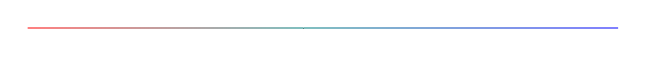
\begin{tikzpicture}
	\fill [left color=red!50, right color=teal!50] (0,0) rectangle (3.5,.01);
	\fill [left color=teal!50, right color=blue!50] (3.5,0) rectangle (7.5,.01);
	\end{tikzpicture}
\vspace{0.5cm}

\begin{definition}
 
Dada una elipse, $\ \frac{x^2}{a^2}+\frac{y^2}{b^2}=1\, \  $ con $\ a^2=b^2+c^2\, , \  $ se llama \emph{\textbf{excentricidad}}, $\boldsymbol{\varepsilon }\, , \ $ al cociente entre la distancia focal, $2c$, y el eje mayor $2a$:

$$\boldsymbol{ \subrayado{ \ \boxed{ \ \varepsilon \ = \ \dfrac {c}{a} \ } \ } } \qquad \qquad \boldsymbol{ 0\ < \ \varepsilon \ < 1 }$$
	
\end{definition}
\underline{Observaciones}:

\begin{itemize}
\item 	$ 0\ < \ \varepsilon \ < 1 \quad $ ya que $\ \varepsilon=\dfrac c a = \dfrac{\sqrt{a^2-b^2}}{a}=\sqrt{1-\dfrac{b^2}{a^2}}$
\item Si $\varepsilon=0 \ \to \ c=0 \ \to \ a=b\ \  \Rightarrow \ $  se obtiene una circunferencia.
\item la elipse se aproxima a la circunferencia a medida que $\varepsilon$ se aproxima a cero \textcolor{gris}{(en cálculo se expresará como $\ \varepsilon \to 0$)}, cuando más se aproxima a uno la excentricidad, la elipse es más achatada.
\end{itemize}

\begin{figure}[H]
	\centering
	\includegraphics[width=.75\textwidth]{img-conicas/conicas25.png}
	\end{figure}

\begin{miejercicio}

Encuentra la ecuación de la elipse que tiene sus focos en $F(5,2)$ y $F'(1,2)$ y pasa por el punto $P(0,2)$. Encuentra su excentricidad.

\rule{250pt}{0.1pt}

\vspace{2mm} El centro de la elipse estará al medio de los focos, $\mathcal O_{
\mathcal E}=\dfrac{F+F'}{2}=(3,2)$, por lo que la ecuación de la elipse tomará la forma: $\ \ \dfrac{(x-3)^2}{a^2}+\dfrac{(y-2)^2}{b^2}=1$

\vspace{2mm} Como la elipse pasa por $P(0,2) \ \to \ $ cuando la $x$ valga $0$ la $y$ valdrá $2$, imponiendo esta condición a nuestra ecuación de la elipse:
$\ \ \dfrac{(0-3)^2}{a^2}+\dfrac{(2-2)^2}{b^2}=1 \ \to \ \dfrac 9{a^2}=1 \ \Rightarrow \ a=3>0$

\vspace{2mm} $c=\dfrac 12 d(F,F')=2 \ \to \ $ relación pitagórica de la elipse, $\ a^2=b^2+c^2 \ \to \ 3^2=b^2+2^2 \ \Rightarrow \ b=\sqrt{5}$

\begin{multicols}{2}
\vspace{2mm} La ecuación de la elipse buscada es: 

\vspace{4mm}$\ \ \dfrac{(x-3)^2}{3^2}+\dfrac{(y-2)^2}{(\sqrt{5})^2}=1$

\vspace{4mm} Finalmente, su excentricidad es: 

\vspace{4mm}$\ \varepsilon=\dfrac{2}{3}=0.67$

\begin{figure}[H]
	\centering
	\includegraphics[width=.4\textwidth]{img-conicas/conicas26.png}
	\end{figure}
\end{multicols}
\end{miejercicio}

\vspace{4mm}
\begin{miejercicio}

Determina la ecuación de la elipse de focos $F'(-1,1)$ y $F(5,1)$ cuya excentricidad es $\varepsilon =3/5$.

\rule{250pt}{0.1pt}

\vspace{2mm} Centro de la elpise, $\mathcal O_{\mathcal E}=M_{FF'}=(2,1);\quad \to \quad \dfrac{(x-2)^2}{a^2}+\dfrac{(y-1)^2}{b^2}=1$

\vspace{2mm} $d(F,F')=6 \ \to \ c=3 ;\quad \varepsilon=\dfrac c a \ \Rightarrow \ \dfrac 3 5 = \dfrac 3 a \ \to \ a=5$

\vspace{2mm} $a^2=b^2+c^2 \ \to \ 5^2=b^2+3^3 \ \Rightarrow \ b=4>0$

\vspace{2mm}	$\dfrac{(x-2)^2}{25}+\dfrac{(y-1)^2}{16}=1$
\end{miejercicio}

\vspace{4mm}
\begin{miejercicio}

Calcula la excentricidad de las siguientes elipses:

\begin{multicols}{2}
\begin{enumerate}[a) ]
\item $\dfrac{x^2}{16}+\dfrac{y^2}{36}=1$
\item $\dfrac{(x+2)^2}{16}+\dfrac{(y-1)^2}{25}=1$	
\item $\dfrac{(x-3)^2}{25}+\dfrac{y^2}{1}=1$
\item $x^2+4y^2=4$
\end{enumerate}	
\end{multicols}

\rule{250pt}{0.1pt}

\vspace{2mm} $\triangleright \ \ a)\quad $ Elipse vertical: $\ a=6,\ b=4 \ \to \ c=\sqrt{6^2-4^2}=2\sqrt{5} \quad \Rightarrow \quad \varepsilon=\dfrac{2\sqrt{5}}{6}=\dfrac{\sqrt{5}}{3}$

\vspace{4mm} $\triangleright \ \ b)\quad $ Elipse horizontal: $\ a=5,\ b=1 \ \to \ c=\sqrt{5^2-1^2}=2\sqrt{6} \quad \Rightarrow \quad \varepsilon=\dfrac{2\sqrt{6}}{5}$

\vspace{4mm} $\triangleright \ \ c)\quad $ Elipse vertical: $\ a=5,\ b=4 \ \to \ c=\sqrt{5^2-4^2}=3 \quad \Rightarrow \quad \varepsilon=\dfrac{3}{5}$

\vspace{4mm} $\triangleright \ \ d)\quad \dfrac{x^2}{4}+\dfrac{y^2}{1}=1 \ \to \ $ Elipse horizontal: $\ a=2,\ b=2 \ \to \ c=\sqrt{2^2-2^2}=\sqrt{3} \quad \Rightarrow \quad \varepsilon=\dfrac{\sqrt{3}}{2}$
	
\end{miejercicio}

%%%
\vspace{4mm}
\begin{miejercicio}

Encuentra fotos, cortes con los ejes y excentricidad de la elipse: $\ \ 16x^2+9y^2=144$

\rule{250pt}{0.1pt}

\vspace{2mm} $16x^2+9y^2=144 \ \to \ \dfrac{16x^2}{144}+\dfrac{9y^2}{144}=1 \ \to \ \dfrac{x^2}{3^2}+\dfrac{y^2}{4^2}=1\ $ Elipse vertical.

\vspace{2mm} $a=4,\ b=3  \ \to \ a^2=b^2+c^2,\ \ 4^2=3^2+c^2 \ \to \ c=\sqrt{7};\quad \varepsilon=\dfrac c a = \dfrac{\sqrt{7}}{4}$

\vspace{2mm} $c=\sqrt{7} \ \to \ F(\sqrt{7},0), \  F'(-\sqrt{7},0)$

\vspace{2mm} Cortes: $ x=0\ \to \ y=\pm 4;\ \ \ y=0 \ \to \ \ x=\pm 3 \quad \Rightarrow \quad (\pm 3,0),\ (0,\pm 4)$
	
\end{miejercicio}

%%%
\vspace{4mm}
\begin{miejercicio}

Encuentra la ecuación de la elipse cuyos vértices son $(\pm 4,0)$ y tiene sus focos en $(\pm 2,0)$. Determina su excentricidad.

\rule{250pt}{0.1pt}

\vspace{2mm} Elipse horizontal: $\ a=4,\ c=2 \ \to \ (a^2=b^2+c^2) \ \to \ b=2\sqrt{3} \ \Rightarrow \ \varepsilon=\dfrac c a=\dfrac 2 4=0.5$

\vspace{2mm} Ecuación de la elipse: $\quad \dfrac{x^2}{16}+\dfrac{y^2}{12}=1$
	
\end{miejercicio}

%%%
\vspace{4mm}
\begin{miejercicio}

Los planetas se mueven en trayectorias elípticas entorno al Sol, estando éste en uno de sus focos (primera ley de Kepler). La distancia más próxima de la Tierra al Sol es de $147\times 10^6$ km y se llama \textbf{\emph{perihelio}}, la distancia de la órbita terrestre más alejada del Sol es el \textbf{\emph{Afelio}} y es de $153\times 10^6$ km. Calcula la ecuación de la órbita terrestre poniendo el origen de coordenadas en el centro y determina la excentricidad de la Tierra.

\rule{250pt}{0.1pt}

\begin{multicols}{2}
Es fácil comprobar que, llamando $\mathcal P$ al perihelio y $\mathcal A$ al afelio, se cumplen las relaciones:

$$\mathcal P\  = \ a-c;\quad \mathcal A\ = \ a+c$$

En millones de kilómetros, $\ \begin{cases} \ 147=a-c\\ 153=a+c \end{cases} \to $

\vspace{2mm}$\to \ 2a=300, \ a=150;\ \ 2c=6,\ c=3$

\vspace{2mm} $a^2=b^2+c^2 \ \to \ b=152.97$ millones de kilómetros.


\begin{figure}[H]
	\centering
	\includegraphics[width=.5\textwidth]{img-conicas/conicas29.png}
	\end{figure}	
\end{multicols}

La ecuación de la órbita terrestre (poniendo el origen de coordenadas en el centro de la elipse) es: $\ \dfrac{x^2}{153^2}+\dfrac{y^2}{152.97}=1\, ; \ \ x$ e $y$ medidos en millones de kilómetros.

\vspace{2mm} Excentricidad de la Tierra: $\quad 	\varepsilon=\dfrac c a =\dfrac 3{150}=0.02$
\end{miejercicio}






%%%%%%%%%%%%%%%%%%%%%%%%%%%%%%%%%%%%%%%%%%%%%%%%%%%%
\vspace{5mm}
\section{Hipérbolas}
\vspace{-5mm}

\begin{tikzpicture}
	\fill [left color=red!50, right color=teal!50] (0,0) rectangle (3.5,.1);
	\fill [left color=teal!50, right color=blue!50] (3.5,0) rectangle (7.5,.1);
	\end{tikzpicture}
\vspace{0.5cm}

\begin{definition}[ Hipérbola]
	
	\textbf{\emph{Hipérbola}:} conjunto de los puntos del plano cuya \underline{diferencia} de distancias a dos puntos fijos llamados \emph{focos}, $\boldsymbol F\ \text{ y } \boldsymbol{F'}$, es un valor constante $\boldsymbol{2a}$.
\end{definition}


La recta que une los focos es el \emph{eje focal}. El punto medio de los focos es el \emph{centro} de la hipérbola y los puntos de intersección de ésta con el eje focal son los \emph{vértices} de la misma.

\vspace{4mm}
\begin{multicols}{2}
$d(P,F')-d(P,F)=2a$

$\sqrt{(x+c)^2+y^2}-\sqrt{(x-c)^2+y^2}=2a$

$\left(\sqrt{(x+c)^2+y^2}\right)^2=\left(2a-\sqrt{(x-c)^2+y^2}\right)^2$

Precediendo como en la elipse,

$$ \boldsymbol{ \dfrac{x^2}{a^2}+\dfrac{y^2}{a^2-c^2}=1 } $$

Ecuación igual a la obtenida para la elipse pero ahora $\boldsymbol{a^2-c^2<0}$ debido a que en el triángulo $PFF'$, $2a$ representa la diferencia de dos lados que siempre ha de ser menor que el tercer lado $2c$ (ver figura)
	\begin{figure}[H]
	\centering
	\includegraphics[width=.4\textwidth]{img-conicas/conicas11.png}
	\end{figure}
\end{multicols}

\begin{footnotesize}
\begin{multicols}{2}
\begin{figure}[H]
	\centering
	\includegraphics[width=.3\textwidth]{img-conicas/conicas12.png}
	\end{figure}	
	\color{gris}
	Es sabido que, en cualquier triangulo, la suma de dos lados es mayor que el tercer lado: 
	
	\vspace{-2mm}
	$\ d'<d+z \ \to \ d'-d<z\, \ $ es decir, la resta de dos lados es mayor que el tercer lado.
\end{multicols}
\end{footnotesize}

\color{black}
\normalsize{Si} $\ a^2-c^2<0 \ \to \ c^2-a^2>0 \ \to \ $
\textbf{llamando $\ \  \boxed{\ \subrayado{\ \boldsymbol { b=\sqrt{c^2-a^2} \ } } \ }\ , \ $} 
podemos escribir: 

$b^2=c^2-a^2 \ \to \ a^2-c^2=-b^2 \quad \Rightarrow \qquad 
\boxed{\
 \subrayado{\  \boldsymbol{ \dfrac{x^2}{a^2}-\dfrac{y^2}{b^2}=1 } \ } \ }\quad $
Ecuación reducida de la hipérbola.

\vspace{4mm}
\underline{Observaciones}:
\vspace{-3mm}
\begin{itemize}

\item La ecuación de la hipérbola es simétrica respecto de $\mathcal O$, de $\mathcal OX$ y de $\mathcal OY$.
\item La distancia entre los focos, situados en $(\pm c,0)$ es $2c$ y se llama distancia focal.
\item Las intersecciones de la hipérbola con el eje focal proporcionan los vértices de la hipérbola, $V(\pm a, 0)$ 
\item La hipérbola no corta al eje $\mathcal OY$
\item El segmento $b$, representado en la figura, junto con el semieje $a$ forman un triángulo rectángulo de hipotenusa $c$. \textcolor{gris}{La relación pitagórica en la hipérbola adopta la forma $\ c^2=a^2+b^2$}
\item Las rectas $\ y=\pm \dfrac b a x\, , \ $ son las \emph{asíntotas} de la hipérbola \textcolor{gris}{(se obtiene fácilmente al sustituir el $1$ por un $0$ en la ecuación de la hipérbola)}.
\end{itemize}

\begin{figure}[H]
	\centering
	\includegraphics[width=.75\textwidth]{img-conicas/conicas30.png}
	\end{figure}


\begin{miejemplo}

Determina los elementos de la hipérbola $\ \dfrac{x^2}4-\dfrac{y^2}5=1$

\rule{250pt}{0.1pt}

\vspace{2mm}
$a^2=4 \to a=2\, ; \ b^2=5\to b=	\sqrt 5 \ \Rightarrow \ c^2=a^2+b^2=9 \to c=3$

\vspace{2mm}Focos en $(\pm 3, 0)$, vértices en $(\pm 2,0)$ y centro en $(0,0)$

\vspace{2mm}Las asíntotas son $ \ y=\pm\dfrac{\sqrt 5}{2}x$
\end{miejemplo}




\vspace{4mm} \underline{Otras posiciones}:
$\qquad \qquad x\ \leftrightarrow \ y \quad \Rightarrow \qquad $ 


\begin{figure}[H]
	\centering
	\includegraphics[width=.95\textwidth]{img-conicas/conicas13.png}
	\end{figure}

\textbf{Hipérbolas desplazadas}:

Hipérbola con centro en $ \mathcal O_{\mathcal H}\, (x_0,y_0) : \qquad $ ${\displaystyle \boxed{ \ \boldsymbol{ {\frac {(x-x_0)^{2}}{a^{2}}}-{\frac {(y-y_0)^{2}}{b^{2}}}=1} } \ } $


\begin{figure}[H]
	\centering
	\includegraphics[width=1\textwidth]{img-conicas/conicas34.png}
	\end{figure}


%\vspace{0.5cm}
\subsection{Excentricidad de la hipérbola}
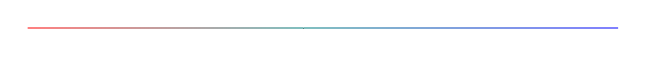
\begin{tikzpicture}
	\fill [left color=red!50, right color=teal!50] (0,0) rectangle (3.5,.01);
	\fill [left color=teal!50, right color=blue!50] (3.5,0) rectangle (7.5,.01);
	\end{tikzpicture}
\vspace{0.5cm}

\begin{definition}
 
Dada una hipérbola, $\ \frac{x^2}{a^2}-\frac{y^2}{b^2}=1\, \  $ con $\ c^2=a^2+b^2\, , \  $ se llama \emph{\textbf{excentricidad}}, $\boldsymbol{\varepsilon }\, , \ $ al cociente entre la distancia focal, $2c$, y el eje mayor $2a$:

$$\boldsymbol{ \subrayado{ \ \boxed{ \ \varepsilon \ = \ \dfrac {c}{a} \ } \ } } \qquad \qquad \boldsymbol{  \varepsilon \ > 1 }$$
	
\end{definition}
\underline{Observaciones}: $\quad $ En la igualdad $\ c^2=a^2+b^2 \, , \  $ dividiendo por $\ a^2\ \to \ \left(\dfrac{c}{a}\right)^2=1+\left(\dfrac{b}{a}\right)^2\, , \ $ por lo que, $\ \boldsymbol{ \varepsilon^2=1+m^2_{asint}}\, \ $ siendo $m_{asint}$ la pendiente de la asíntota. De esta relación podemos asegurar que \emph{cuanto mayor sea la pendiente de la asíntota, $b/a$, mayor será la excentricidad $c/a$ de la hipérbola.} 


\begin{figure}[H]
	\centering
	\includegraphics[width=.9\textwidth]{img-conicas/conicas31.png}
	\end{figure}

\vspace{4mm}
\begin{miejemplo}
	
	Determina los elementos y excentricidad de las elipses:
	
	\vspace{2mm}$a)\ \ \dfrac{x^2}{25}-\dfrac{y^2}{16}=1;\qquad \qquad b)\ \ 3y^2-4x^2=12$
	
	\vspace{6mm} $\triangleright \ \ a)\quad a=5,\ b=4 \ \to \ c^2=a^2+b^2 ,\ \ c=\sqrt{41};\quad \varepsilon=\dfrac c a = \dfrac {\sqrt{41}}{5}=1.28$
	
	\vspace{2mm} Focos en $\ (\pm \sqrt{41},0)$, $\quad$ Vértices en $\ (\pm 5,0)$
	
	\vspace{2mm} Asíntotas: $\ y=\pm \dfrac b a \, x=\pm \dfrac 45\, x$
	
	\vspace{6mm} $\triangleright \ \ b)\quad 3y^2-4x^2=12\, , \ \text{ dividiendo por } 12 \  \ \to \ \dfrac{y^2}{4}-\dfrac{x^2}{3}=1$
	
	\vspace{2mm} $a=2,\ b=\sqrt{3} \ \to \ c^2=a^2+b^2 , \ \ c=\sqrt{7};\quad \varepsilon =\dfrac c a = \dfrac {\sqrt{7}}{2}=1.32$
	
	\vspace{2mm} Focos en $\ (0,\pm \sqrt{7});\quad$ Vértices en $\ (0,2)$. $\qquad $ Asíntotas: $\ y=\pm \dfrac a b \, x= \pm \dfrac{2\sqrt{3}}{3}\, x$
\end{miejemplo}
\vspace{5mm}

%%%
\begin{miejercicio}

Encuentra la ecuación de la hipérbola centrada en el origen cuyas asíntotas son $y=\pm \dfrac 1 5 \, x$ y tiene un vértice en $V(2,0)$. Determina, también, su excentricidad.
\rule{250pt}{0.1pt}

\vspace{2mm}
	
\end{miejercicio}


%%%
\begin{miejercicio}

Ecuación reducida de la hipérbola que pasa por el punto $P(2,1)$ y tiene por asíntotas $y=\pm 3 x$. Determina, también, su excentricidad.

\rule{250pt}{0.1pt}

\vspace{2mm} $V(2,0) \ \to \ a=2;\quad $ Asíntotas $\ \dfrac b a = \dfrac 1 5 \ \to \ \dfrac b 2=\dfrac 1 5 \ \to \ b=\dfrac 2 5; \quad c^2=a^2+b^2 \ \to \ c=\dfrac{2\sqrt{26}}{5}$  

\vspace{2mm}$\varepsilon = \dfrac c a = \dfrac {\sqrt{26}}{5}=1.02;\quad $ Focos: $\ (\pm 2\sqrt{26}/5, 0);\quad$ Vértices $\ (\pm 2, 0)$
	
\end{miejercicio}


%%%
\begin{miejercicio}

Ecuación de la hipérbola de focos en $(\pm 3,0)$, con excentricidad $\varepsilon=3$.

\rule{250pt}{0.1pt}

\vspace{2mm} $c=3 \ \to \ \varepsilon=3=\dfrac c a =\dfrac 3 a \ \to \ a=1;\quad c^2=a^2+b^2 \ \to \ b=2\sqrt{2} \ \Rightarrow \ \dfrac{y^2}{8}-\dfrac{x^2}{1}=1$ 

\vspace{2mm} \textcolor{gris}{ Focos en $\ (0,\pm 3)\quad $ Vértices en $\ (0,\pm 1)\quad $ Asíntotas: $\ y=\pm \dfrac a b \, x = \dfrac {\sqrt{2}}{4}\, x$}
	
\end{miejercicio}


%%%
\begin{miejercicio}

Ecuación de la hipérbola de focos en $(\pm 3,0)$ y que tiene por asíntotas las rectas de ecuaciones $y=\pm \dfrac{2\sqrt{5}}{5}\, x$

\rule{250pt}{0.1pt}

\vspace{2mm} $c=3 \, ; \quad \dfrac b a =\dfrac {2\sqrt{5}}{5}= \dfrac {2}{\sqrt{5}} \quad \to \quad c^2=a^2+b^2 \to \  \cdots \cdots \ \to \ a=\sqrt{5},\ b=2$

\vspace{2mm} $\dfrac{x^2}{5}-\dfrac{y^2}{4}=1 \qquad $ \textcolor{gris}{Vértices $\ (\pm 2, 0); \quad \varepsilon=\dfrac ca=\dfrac{3\sqrt{5}}{5}=1.34$ }
	
\end{miejercicio}




%%%
\begin{miejercicio}

Determina los elementos y excentricidad de las elipses:
	
	\vspace{2mm}$a)\ \ \dfrac{x^2}{36}-\dfrac{(y-1)^2}{64}=1\, ; \qquad \qquad b)\ \ \dfrac{(y-1)^2}{16}- \dfrac{(x-1)^2}{9}=1$

\rule{250pt}{0.1pt}

\vspace{4mm}$\triangleright \quad a)\ \ \mathcal O_{\mathcal H}\ (0,1);\ \quad a=6,\ b=8 \ \to \ c^2=a^2+b^2 \ \to\ c=10$

\vspace{2mm}$ V(\pm 6,1);\ \ F(\pm10,1)\ \ \text{asíntotas}:\ y-1=\pm \dfrac 8 6 \, x$

\vspace{6mm}$\triangleright \ \ b)\quad \mathcal O_{\mathcal H}\ (0,1);\ \quad a=4,\ b=3 \ \to \ c^2=a^2+b^2\ \to \ c=5$

\vspace{2mm} $F(1,6),\ F(1,-4);\ \ \ V(1,5),\  V'(1,-3);\quad \varepsilon=c a=\dfrac 5 4=1.25;\quad \text{asint.}:\ y-1=\pm \dfrac 4 3 (x-1)$

\begin{figure}[H]
	\centering
	\includegraphics[width=.8\textwidth]{img-conicas/conicas32.png}
	\end{figure}
	
\end{miejercicio}


\vspace{5mm}

\begin{myalertblock}{Como dibujar una hipérbola}
\vspace{2mm}
\begin{enumerate}
\item Trazar la caja central. Éste es el rectángulo con centro en el origen, con lados paralelos a los ejes, que cruza un eje en $\pm a$ y el otro en $\pm b$.
\item Trazar las asíntotas. Éstas son las rectas obtenidas al prolongar las diagonales de la caja central.
\item Determinar los vértices. Estos son los dos puntos de intersección en $x$ o los dos puntos de intersección en $y$.
\item Trazar la hipérbola. Empiece en un vértice, y trace una rama de la hipérbola, aproximando las asíntotas. Trace la otra rama en la misma forma.
\end{enumerate}
\begin{figure}[H]
	\centering
	\includegraphics[width=.6\textwidth]{img-conicas/conicas35.png}
	\end{figure}
\vspace{2mm}
\end{myalertblock}

\vspace{7mm}
\begin{myexampleblock}{Hipérbola equilátera}

\begin{figure}[H]
	\centering
	\includegraphics[width=1\textwidth]{img-conicas/conicas38.png}
	\end{figure}	
	
\vspace{2mm} Se llama así a la hipérbola en la que $a=b \quad \Rightarrow \quad \boldsymbol{x^2-y^2=a^2}$ 

\vspace{2mm} por lo que su excentricidad será $\ \varepsilon=\dfrac c a=\dfrac{\sqrt{a^2+a^2}}{a}=\dfrac{a\sqrt{2}}{a}=\sqrt{2}$

\vspace{2mm} y las asíntotas: $\ y=\pm \dfrac a a x = \pm x$, que son ortogonales (bisectrices de los cuadrantes).

\vspace{2mm} Sería interesante hacer coincidir a las asíntotas con los ejes $\ \Rightarrow \ $ se trata de un giro de $45^o$ respecto del origen de coordenadas.

\vspace{2mm} En estas condiciones, la ecuación resultante puede escribirse como: $\ \boldsymbol{x\, y\ = \ \dfrac {a^2}{2} \ = \ k}$.	

\color{gris}
\vspace{6mm} $y=\dfrac 1 x \ \to \ 1=\dfrac {a^2}{2} \ \to \ a=\sqrt{2}=b \ \to \ c=2;\quad \varepsilon=\sqrt{2};\quad y=\pm x$

\vspace{2mm}  Los focos y los vértices estarán a distancias $c=2$ y $a=1$, pero girados $45^o$. Es fácil comprobar (calcular) que los puntos sobre las bisectrices a estas distancias del origen son: $\ \ F(\sqrt{2},\sqrt{2}),\ F'(-\sqrt{2},-\sqrt{2}),\ V(1,1) \ \text{ y } \ V'(-1,-1)$ 

\vspace{2mm} En la figura de la hipérbola $y=1/x$ se ha llamado $C$ y $C'$ a los focos y $A$ y $A'$ a los vértices.
\color{black}
\vspace{2mm}
\end{myexampleblock}



%%%%%%%%%%%%%%%%%%%%%%%%%%%%%%%%%%%%
\vspace{10mm}
\section{Parábola}
\vspace{-5mm}

\begin{tikzpicture}
	\fill [left color=red!50, right color=teal!50] (0,0) rectangle (3.5,.1);
	\fill [left color=teal!50, right color=blue!50] (3.5,0) rectangle (7.5,.1);
	\end{tikzpicture}
\vspace{0.5cm}


\vspace{5mm}
\begin{definition}[ Parábola]
	
	\textbf{\emph{Parábola}:} conjunto de los puntos del plano  que equidistan de un punto fijo llamado \emph{foco} $\boldsymbol F$ y de una recta fija llamada \emph{directriz} $\boldsymbol d$	
\end{definition}

\vspace{5mm}
\begin{multicols}{2}
$\quad$

A medida que $F$ se acerca a $d$, la parábola se estrecha. Si $F\in d \to $ la parábola se convierte en una recta que pasa por $F$ y es perpendicular a $d$, se trata de un caso de \emph{cónica degenerada}. En lo que sigue consideraremos $F \notin d$.
\begin{figure}[H]
	\centering
	\includegraphics[width=.3\textwidth]{img-conicas/conicas02.png}
	\end{figure}	
\end{multicols}

El caso más sencillo se obtiene cuando el foco $F$ está en uno de los ejes coordenados y la directriz $d$ es perpendicular a ese eje. Supongamos $\ F(0,p)\ $, en el eje $\mathcal OY^+$ y $\ d:y=-p$, paralela al eje $\mathcal OX$. En este caso:

\vspace{4mm}
\begin{multicols}{2}
\begin{figure}[H]
	\centering
	\includegraphics[width=.45\textwidth]{img-conicas/conicas03.png}
	\end{figure}
$\triangleright\  d(P,F)=$

$=\sqrt{(x-0)^2+(y-p)^2}=\sqrt{x^2+(y-p)^2}$	

$\triangleright\ d(P,d)=$

$=\sqrt{(x-x)^2+(y-(-p))^2}=\sqrt{(y+p)^2}$

$d(P,F)=d(P,d) \Rightarrow x^2+(y-p)^2=(x+p)^2$
\end{multicols}

$x^2+\cancel{y^2}+\cancel{p^2}-2yp=\cancel{y^2}+\cancel{p^2}+2yp  \quad \to \qquad \boxed{ \ \subrayado{ \ \boldsymbol{x^2 \, = \, 4py} \ } \ }$ 

\vspace{4mm} \underline{Observaciones}:
\begin{itemize}
\item La ecuación de la parábola, $x^2=4py$, pone de manifiesto que la parábola es simétrica respecto del \emph{eje de la parábola}, recta perpendicular a la directriz que pasa por el foco (en este caso, el eje $\mathcal OY$). 
\item La parábola corta a su eje en el \emph{vértice}, $V(0,0)$.
\item La cantidad $p$ recibe el nombre de \emph{distancia focal} de la parábola. El foco se encuentra en la posición $F(0,p)$
\item La directriz es la recta $y=-p$
\end{itemize}

\vspace{5mm} \underline{Otras posiciones}:
 
 Si $F(0,-p)$ y $d:\ y=+p \ \to \ $ parábola (vertical) hacia abajo: $\ x^2=-4py$

$x\ \leftrightarrow \ y \quad \Rightarrow \qquad $ parábolas horizontales: $\quad \begin{cases} 
\ F(p,0);\ \ \ d:\, x=-p \ \to \ y^2=\ \, 4px \\
\ F(-p,0);\ d:\, x=+p \ \to \ y^2=- 4px \\
\end{cases}$


\begin{figure}[H]
	\centering
	\includegraphics[width=.75\textwidth]{img-conicas/conicas04.png}
	\end{figure}

\begin{miejemplo}

Encuentra el foco y la directriz de la parábola $\ y^2\, =\, 5\, x$


  
\vspace{2mm}

\begin{multicols}{2}
La parábola es horizontal y dirigida hacia $\mathcal OX^+$. 

Como $4p=5 \ \to \ p=5/2$, por lo que el foco está en $F(5/2,0)$ y la directriz es la recta vertical $x=-5/2$. 

El vértice está en el origen de coordenadas, $V(0,0)$.	
\begin{figure}[H]
	\centering
	\includegraphics[width=.25\textwidth]{img-conicas/conicas05.png}
	\end{figure}	
\end{multicols}
\end{miejemplo}

\vspace{5mm}

\begin{theorem}[ Excencentricidad de la parábola]

$\qquad \varepsilon \ \dfrac c a\, ; \quad c=d(P,F);\ \ a=d(P,d) \quad \Rightarrow \quad \varepsilon=1 \, , \quad \forall	 $ parábola.

\vspace{4mm} $\qquad$ \textcolor{gris}{Por definición de parábola, $d(P,F)=d(P,d) \ \to \varepsilon=1$ \QED}
\end{theorem}




\vspace{5mm}
\textbf{Parábolas desplazadas}: $\qquad \boxed{ \ \boldsymbol{(x-x_0)^2\ = \ 4p\, (y-y_0)} \ } $

\begin{multicols}{2}


Desarrollando: 

$x^2-2x_0x+x_0^2=4py-4py_0 \ \to $

$\to \ y=\dfrac 1{4p}\, x^2-\dfrac{x_0}{2p}\, x+\dfrac{x_0^2+4py_0}{4p}$

\vspace{1mm} Llamando $\quad a=\dfrac 1{4p}\; \ b=\dfrac{x_0}{2p};\ c= \dfrac{x_0^2+4py_0}{4p}$

\vspace{1mm} Podremos escribir la parábola como 

$$\boldsymbol{y=ax^2+bx+c}$$
\begin{figure}[H]
	\centering
	\includegraphics[width=.4\textwidth]{img-conicas/conicas36.png}
	\end{figure}	
\end{multicols}		

Veamos ahora como dada la parábola $y=ax^2+bx+c$ podemos encontrar su vértice $V$ y su distancia focal $p$:

Despejando $p$ de la definición de $a:\qquad \boldsymbol{ p=\dfrac 1{4a} }$

Despejando $x_0$ de la definición de $b:\qquad x_0=-2pb=-2p\dfrac{1}{4a}=-\dfrac{b}{2a}$

Despejando $y_0$ de la definición de $c:\qquad y_0=\dfrac{4pc-x_0^2}{4p}=\dfrac{4\dfrac{1}{4a}c-\left(-\dfrac{b}{2a} \right)^2}{4\dfrac{1}{4a}}=\dfrac{\dfrac c a - \dfrac{b^2}{4a^2}}{\dfrac 1 a}=\dfrac{4ac-b^2}{4a}$

\begin{adjustwidth}{25pt}{25pt}
\begin{destacado}	
Dada $\boldsymbol{ y=ax^2-bx+c} \ \Rightarrow \ $ el vértice está en $\ \boldsymbol {V\left( -\dfrac{b}{2a} \, , \, \dfrac{4ac-b^2}{4a} \right) } $
\end{destacado}
\end{adjustwidth}

\textcolor{gris}{Lo más sencillo es recordar que la abcisa del vértice de la parábola está en $x_0=-\frac{b}{2a}$ y, para encontrar la ordenada del vértice, $y_0$, sustituir el valor de $x_0$ el la ecuación de la parábola $(y=ax^2+bx+c)$}

\vspace{5mm}
\begin{miejercicio}

Determina los elementos de la parábola $\ (x-1)^2=-6(y+4)$

\rule{250pt}{0.1pt}

\vspace{2mm} 

\begin{multicols}{2}
Comparando con $(x-x_0)^2=-4p(y-y_0) \ \to \ x_0=1,\ y_0=-4,\ p=\dfrac 6 4 = \dfrac 3 2$

\vspace{3mm} Tenemos una parábola vertical hacia abajo con vértice en $V(1,-4)$, foco en $F(1,-4-3/2)=(1,-11/2)$ y directriz $y=-4+3/2=-5/2$. 

\vspace{3mm}El eje de simetría es la recta vertical $x=1$ y, obviamente, $\varepsilon=1$ al tratarse de una parábola.
\begin{figure}[H]
	\centering
	\includegraphics[width=.5\textwidth]{img-conicas/conicas37.png}
	\end{figure}	
\end{multicols}	
	
\end{miejercicio}

\vspace{5mm}
\begin{miejercicio}

Determina los elementos de la parábola $\ y=-\dfrac 16\, x^2 +\dfrac 1 3 x -\dfrac {25}{6}$

\rule{250pt}{0.1pt}

\vspace{4mm} Teóricamente: $p=\dfrac 1{4|a|}=\dfrac{1}{4(1/6)}=\dfrac 3 2$

\vspace{2mm} $x_0=-\dfrac{b}{2a}=-\dfrac{1/3}{2 (1/6)}=1;\quad y_0=\dfrac{4ac-b^2}{4a}=\dfrac{4(-1/6)(-25/6)-1/9}{4(-1/6)}=\dfrac{25/9-1/9}{-2/3}=-4$

\vspace{2mm} El vértice está en $\ V(1,-4)$, el foco en en $F(1,-4-3/2)=(1,-11/2)$ y la directriz $y=-4+3/2=-5/2$.  El eje de simetría es la recta vertical $x=1$ y, obviamente, $\varepsilon=1$ al tratarse de una parábola \textcolor{gris}{(ver figura del ejercicio anterior)}.

\vspace{2mm}\begin{small} \textcolor{gris}{También podríamos haber obtenido $y_0$ al sustituir $x=1$ en la ecuación  $y=-1/6\, x^2 + 1/3\,  x -{25}{6}$}\end{small}

\vspace{6mm} Completando cuadrados:

\vspace{2mm} $\ 6y=-x^2+2x-25 ; 6y= -(x^2-2x+1)+1-25=-(x-1)^2-24 \ \to \ 6y+24=(x-1)^2 \ \to \ 6(y+4)=-(x^2-1) \ \Rightarrow \ (x-1)^2=-6(y+4) \ $ que es la parábola del ejercicio anterior.
	
\end{miejercicio}


\vspace{5mm}

\begin{myalertblock}{Diámetro focal}

Podemos usar las coordenadas del foco para estimar el ``ancho'' de una parábola cuando tracemos su gráfica. El segmento de recta que pasa por el foco y es perpendicular al eje, con puntos extremos en la parábola, se llama \emph{lado recto}, y su longitud es el \emph{diámetro focal} de la parábola.
	\begin{multicols}{2}
		\begin{figure}[H]
			\centering
			\includegraphics[width=.3\textwidth]{img-conicas/conicas39.png}
			\end{figure}
		
		En la  figura adjunta podemos ver que la distancia de un punto extremo $Q$ del lado recto a la directriz también es  $|2p|$. En consecuencia, la distancia de $Q$ al foco también debe ser $|2p|$ (por la definición de una parábola), de modo que el diámetro focal es $|4p|$. 
	\end{multicols}	
\end{myalertblock}

\vspace{5mm}

\begin{miejercicio}

\begin{multicols}{2}
Determina los elementos de la parábola $6x+y^2=0$. Encuentra, también, el diámetro focal.

\rule{150pt}{0.1pt}

	\vspace{2mm} $y=2=-6x =4px \ \to \ p=-3/2$
	
	\vspace{2mm} $F(-3/2,0);\quad $ directriz: $\ x=3/2$
	
	\vspace{2mm} Parábola horizontal hacia la izquierda.
	
	\vspace{2mm} Diámetro focal: $\ |4p|=6\,\mathrm{u}$
	\begin{figure}[H]
			\centering
			\includegraphics[width=.35\textwidth]{img-conicas/conicas40.png}
	\end{figure}
\end{multicols}
	
\end{miejercicio}

\begin{miejercicio}

\begin{multicols}{2}
\begin{small} En un puente colgante, la forma de los cables de suspensión es parabólica. El puente que se muestra en la figura tiene torres que están a $600$ m una de la otra, y el punto más bajo de los cables de suspensión está a $150$ m debajo de la cúspide de las torres. Encuentre la ecuación de la parte parabólica de los cables, colocando el origen del sistema de coordenadas en el vértice.	\end{small}
\begin{figure}[H]
			\centering
			\includegraphics[width=.4\textwidth]{img-conicas/conicas41.png}
	\end{figure}
\end{multicols}
 
\vspace{2mm} La parábola $x^2=4py$ pasará por el punto $(600,150)$

\vspace{2mm} $600^2=4p\cdot 150 \ \to \ p=600 \quad \Rightarrow \quad x^2=2400 y$
\end{miejercicio}

\vspace{5mm} \textbf{Parábolas desplazadas} $\qquad \quad \boldsymbol{(x-x_0)^2 \ = \ 4p\, (y-y_0)}$

\vspace{5mm} 
\begin{miejercicio}

Encuentra los elementos de la parábola $\ x^2-4x=8y-28$

\rule{250pt}{0.1pt}

\begin{multicols}{2}
\vspace{2mm}	Completando cuadrados: $\ \  (x-2)^2-4=8y-28 \ \to \ \boldsymbol{(x-2)^2} \ =8y-24 =\ \boldsymbol{ 8(y-3)}$

\vspace{2mm} Luego $\ 4p=8 \ \to \ p=2$, por lo que

\vspace{2mm} Se trata de una parábola vertical hacia arriba con centro (vértice) en $V(2,3)$. El foco estará $p=2$ unidades encima del vértice: $\ F(2,5)$ y la directriz estará $p=2$ unidades hacia abajo del vértice, se tratará de la recta $y=1$

\begin{figure}[H]
			\centering
			\includegraphics[width=.4\textwidth]{img-conicas/conicas42.png}
	\end{figure}
\end{multicols}
\end{miejercicio}

\begin{center} \rule{250pt}{0.2pt} \end{center}	

\vspace{5mm}

\begin{cuadro-naranja}
\textcolor{blue}{RESUMEN:}
\vspace{-3mm}
\begin{figure}[H]
	\centering
	\includegraphics[width=.95\textwidth]{img-conicas/conicas14.png}
	\end{figure}
\end{cuadro-naranja}

\vspace{5mm}

\begin{center} \rule{250pt}{0.2pt} \end{center}	


\vspace{1cm}
\section{Tangentes a cónicas}

\begin{tikzpicture}
	\fill [left color=red!50, right color=teal!50] (0,0) rectangle (3.5,.1);
	\fill [left color=teal!50, right color=blue!50] (3.5,0) rectangle (7.5,.1);
	\end{tikzpicture}
\vspace{0.5cm}

Una cónica es una ecuación de segundo grado y una recta lo es de primer grado. Las disponemos en forma de sistema de ecuaciones para ver que puntos tienen en común y al despejar $y$ en la recta y sustituir en la cónica se obtendrá una ecuación de segundo grado en $x, \ \alpha x^2+\beta x-\gamma=0, $ que pude tener, según su discriminante, $\Delta=\beta^2-4\alpha \beta$, dos soluciones (recta y cónica secantes), una solución (tangentes) o ninguna solución (recta exterior a la cónica).

De este modo, si queremos que a recta que pase por el punto $P(x_0,y_0)$ sea \textbf{tangente} a nuestra cónica, tenemos que exigir que el discriminante de la ecuación de segundo grado a la que lleguemos al resolver el sistema sea cero, es decir, $\boldsymbol{\Delta=0}$. Nuestra incógnita va a ser la pendiente, $\boldsymbol{m}$ de la recta tangente.

\vspace{5mm}
\textbf{Recta tangenta a una cónica en el punto $\boldsymbol{P(x_0,y_0)}$}
\begin{table}[H]
\centering
\begin{tabular}{ccccc}
Elipse & $\quad$ & Hipérbola & $\quad$ & Parábola \\ \cline{1-1} \cline{3-3} \cline{5-5}  \\
$ \begin{cases} \ \dfrac{x^2}{a^2}+\dfrac{y^2}{b^2}=1 \\ \ y-y_0=m(x-x_0)  \\ \qquad \Delta=0 \end{cases}$ &         & $ \begin{cases} \ \dfrac{x^2}{a^2}-\dfrac{y^2}{b^2}=1 \\ \ y-y_0=m(x-x_0) \\ \qquad \Delta=0 \end{cases}$ &         & $ \begin{cases} \ y^2=4px \\ \ y-y_0=m(x-x_0) \\ \qquad \Delta=0 \end{cases}$
\end{tabular}
\end{table}

\vspace{5mm}

\begin{miejercicio}

Encontrar la ecuación de la recta tangente a la cónica $\dfrac {x^2}{18}+\dfrac{y^2}{9}=1$ que pasa por el punto $P(4,1)$.

\rule{250pt}{0.1pt}

\vspace{2mm}
$E:\ \ \dfrac {x^2}{18}+\dfrac{y^2}{9}=1 \ \leftrightarrow \ x^2+2y^2=18\, ; \qquad R.T. \ \ P(4,1)$

$P(4,1)\ \in \ E \, : \quad \dfrac {4^2}{18}+\dfrac{1^2}{9}=1 \ \to \ \dfrac {16}{18}+\dfrac{1}{9}=\dfrac{18}{18}=1	$

\vspace{2mm} Puesto que el punto de tangencia es un punto de la recta buscada, su ecuación será de la forma:
$\ y-1=m(x-4)\ $

\vspace{2mm} Por otra parte, como la recta buscada es la recta \emph{tangente} a la elipse, el sistema de ecuaciones formado por la ecuación de la elipse y la de la recta ha de tener \emph{solución única}, el punto de tangencia.
$\ \ \ \begin{cases}
\ \dfrac {x^2}{18}+\dfrac{y^2}{9}=1 & \quad (1)\\
\ y-1=m(x-4) & \quad (2)
\end{cases}$

\vspace{2mm} Sustituyendo $\ (1)\ $ en $\ (2)\, :\qquad x^2+2(mx-4m+1)^2=18$

\vspace{2mm}  $(1+2m^2)x^2+(4m-16m^2)x+32m^2-16m+16=0$

\vspace{2mm}  Para que esta ecuación de segundo grado \textcolor{gris}{$(ax^2+bx+c=0)$} tenga solución única es necesario que su \emph{discriminante} sea cero \textcolor{gris}{$(\Delta=b^2-4ac=0)$}.

\vspace{2mm}  $\Delta=0 \ \to \ (4m-16m^2)^2-4(1+2m^2)(32m^3-16m-16)=0 \ \to $

\vspace{2mm}  $\to \ \cancel{256m^4}- \bcancel{128m^3}+16m^2-( \cancel{256m^4}-\bcancel{128m^3}-64m-64)=0  \ \to $

\vspace{2mm}  $\to  16m^2+66m+64=0 \ \to \ m^2+4m+4=0 \ \to \ (m+2)^2=0 \ \to \ \boldsymbol{m=-2}$

\vspace{2mm}  Conocida la pendiente, la recta tangente buscada es: $\ y-1=-2(x-4) \ \to \ \boldsymbol{2x+y=9}$
\end{miejercicio}

\begin{figure}[H]
			\centering
			\includegraphics[width=.6\textwidth]{img-conicas/conicas44.png}
	\end{figure}

\begin{miejercicio}

Encuentra la recta tangente y normal a las siguientes cónicas en los siguientes puntos:

\vspace{2mm} $a)\ \ \dfrac{x^2}{9}+\dfrac{y^2}{4}=1	;\ P(5,0);\qquad b)\ \ x^2-y^2=16;\ P(0,2);\qquad c)\ \ y^2=2x;\ P(-1,0)$

\rule{250pt}{0.5pt}

\vspace{4mm} \begin{small} $\triangleright \ \ a)\quad \begin{cases} \ \dfrac{x^2}{9}+\dfrac{y^2}{4}=1 \\ \ y=m(x-5) \\ \qquad (\Delta=0) \end{cases} \to \dfrac{x^2}{9}+\dfrac{(m(x-5))^2}{4}=1	\ \to \ (4+9m^2)x^2-90m^2 x+(225m^2-36)=0$ \end{small}

\vspace{2mm} $\Delta = 0 \ \to \ (-90m^2)^2-4(4+9m^2)(225-36m^2)=0 \ \to \ 16m^2=4 \ \Rightarrow \ m=\pm \dfrac 1 2$

\vspace{2mm} Hay dos soluciones:  $\quad y=\pm \dfrac 1 2 \, (x-5)$

\vspace{4mm} $\triangleright \ \ b)\quad \begin{cases} \ x^2-y^2=16 \\ \ y-2=mx \\ \quad (\Delta=0) \end{cases} \to \cdots  \Delta=0 \cdots \to m=\pm \dfrac{\sqrt{5}}{2}$ 

\vspace{2mm} Hay dos soluciones: $\quad y=\pm \dfrac{\sqrt{5}}{2}\, x + 2$ 

\vspace{4mm} $\triangleright \ \ c)\quad \begin{cases} \ y^2=2x \\ y=m(x+1) \\ \quad (\Delta=0) \end{cases} \to \cdots  \Delta=0 \cdots \to m=\pm \dfrac{\sqrt{2}}{2}$ 
 

\vspace{2mm} Hay dos soluciones: $\quad y=\pm \dfrac{\sqrt{2}}{2}(x+1)$ 
\end{miejercicio}

Las rectas normales se obtienen fácilmente al exigir que $m_N=-\dfrac 1{m_T}$, siendo $m_T$ la pendiente de la recta tangente y $m_N$ la de la recta normal.

\begin{figure}[H]
			\centering
			\includegraphics[width=1\textwidth]{img-conicas/conicas43.png}
	\end{figure}



\vspace{.5cm}
\section{Clasificación de las cónicas}

\begin{tikzpicture}
	\fill [left color=red!50, right color=teal!50] (0,0) rectangle (3.5,.1);
	\fill [left color=teal!50, right color=blue!50] (3.5,0) rectangle (7.5,.1);
	\end{tikzpicture}
\vspace{0.5cm}


\textbf{Por su discriminante}


Una sección cónica puede ser definida por un polinomio de segundo grado con dos variables:

$$\ Ax^2 + Bxy + Cy^2 + Dx + Ey + F= 0\, ,\ $$

se llama  \emph{\textbf{discriminante} de la cónica} a la cantidad  $\quad   \boxed{ \ \subrayado{ \ \boldsymbol{ \Delta \ = \ B^2 - 4AC } \ } \ } $

\vspace{4mm} \underline{El discriminante determina la forma de la sección cónica}

\begin{itemize}
\item	$\Delta < 0  \ \Rightarrow \ $  la ecuación describe una elipse o una circunferencia.
\item $\Delta =0 \ \Rightarrow \ $ la ecuación describe una parábola.
\item $\Delta >0 \ \Rightarrow \ $ la ecuación describe una hipérbola.
\end{itemize}


. Si el discriminante es igual a 0, la ecuación describe una parábola. Si por el contrario es mayor a cero, la ecuación describe una hipérbola. 

\vspace{5mm}
\textbf{Por su excentricidad}

\begin{itemize}
\item La excentricidad de una circunferencia es $0\ \  (\varepsilon = 0)$.
\item La excentricidad de una elipse es mayor que cero y menor que uno $\ \ (0 < \varepsilon < 1)$.
\item La excentricidad de una parábola es $1\ \  (\varepsilon = 1)$.
\item La excentricidad de una hipérbola es mayor que $1\ \  (\varepsilon > 1)$.	
\end{itemize}


\vspace{5mm}

\begin{miejemplo}

Clasifica las siguientes cónicas:

\vspace{2mm} $a)\ \ x^2+2xy-y^2-x+3y-6=0;\qquad b)\ \ x^2+6y+13=0;\qquad c)\ \ x^2+y^2-6x+8y-25=0$

\vspace{2mm} $d)\ \ 4y^2-x^2=4;\qquad e)\ \ 5x^2+8y^2=7$

\vspace{15mm} $\triangleright\ \ a) \quad  x^2+2xy-y^2-x+3y-6=0 \ \to \ A=1;\ B=2;\ \ C= -1 \ \Rightarrow  \ \Delta=B^2-4AC=2^2-4(1)(-1)=8>0 \ \to \ $ Hipérbola


\vspace{5mm} $\triangleright\ \ b) \quad x^2+6y+13=0 \ \to \ A=1;\ B=0;\ C=0 \ \to \ Delta=0 \ \to \ $ Parábola.


\vspace{5mm} $\triangleright\ \ c) \quad x^2+y^2-6x+8y-25=0 \ \to \ A=1;\ B=0;\ C=1 \ \to \ \Delta=-4<0 \ \to \ $ Circunferencia o Elipse:

\vspace{2mm} Completando cuadrados: $\ (x-3)^2-9+(y+4)^2-16-25=0 \ \to \ (x-3)^2+(y+4)^2=50 \ \Rightarrow \ $ Circunferencia de centro $(3,-4)$ y radsior $\sqrt{50}\ \mathrm{u}$.

\vspace{5mm} $\triangleright\ \ d) \quad 4y^2-x^2-4=0 \ \to A=-1;\ B=0;\ C=4 \ \to \ \Delta=16>0 \ \to \ $ Hipérbola


\vspace{5mm} $\triangleright\ \ e) \quad 5x^2+8y^2-7=0 \ \to \ A=5;\ B=0;\ C=8 \ \to \ \Delta=-160<0 \ \to \   $ Circunferencia o Elipse:

\vspace{2mm} Dividiendo por $7 \quad \to \quad \dfrac{x^2}{7/5}+\dfrac{y^2}{7/8}=1 \ \to \ $ Elipse.
	
\end{miejemplo}

\vspace{5mm}
\begin{miejercicio}

Clasifica las siguientes cónicas y determina sus elementos:

\vspace{2mm} $a)\ \ x^2+y^2-2x-2y+1=0;\qquad b)\ \ 2x^2+2y^2-4x-4y+19=0;\qquad c)	\ \ x^2+4y^2=100;$

\vspace{2mm} $d)\ \ 8x^2-3y^2=120;\qquad e)\ \ y^2=6x;\qquad f)\ \ y=x^2-2x+3;\qquad g)\ \ x=-3y^2+y+8$

\rule{250pt}{0.1pt}

\vspace{5mm} $\triangleright\ \ a) \quad  x^2+y^2-2x-2y+1=0 \ \to \ \Delta=-4<0\ \to \ $ Circunferencia o Elipse. 

\vspace{2mm} Completando cuadrados: $(x-1)^2-1+(y-1)^2-1+1=0 \ \to \ (x-1)^2+(y-1)^2=1\quad $ Circunferencia de centro $(1,1)$ y radio $1\, \mathrm{u}$.


\vspace{5mm} $\triangleright\ \ b) \quad 2x^2+2y^2-4x-4y+19=0 \ \to \ \Delta= -16<0 \ \to \ $ Circunferencia o Elipse. 

\vspace{2mm}  Dividimos por $2,\ \ x^2+y^2-2x-2y+19/2=0 \ \to \ $  Completando cuadrados: $ (x-1)^2-1+(y-1)^2-1+19/2=0 \ \to \ (x-1)^2+(y-1)^2=-15/2\quad$ No se corresponde con ninguna cónica \textcolor{gris}{$\big(\nexists \mathcal R=\sqrt{-15/2}\big)\ \ $ Además, la solución es el conjunto vacío, $\emptyset$, mo existe ningún punto del plano que verifique esta ecuación, la suma de dos cuadrados jamás dará una cantidad negativa. }.

\vspace{5mm} $\triangleright\ \ c) \quad x^2+4y^2-100=0\ \to \ \Delta=-16<0 \ \to \  $  Circunferencia o Elipse. 

\vspace{2mm} $A\neq C \ \to \  $ Dividiendo por 100, $\ \dfrac{x^2}{10^2}+\dfrac{y^2}{5^2}=1 \ \to \ $ Se trata de una Elipse centrada en el origen con semiejes $a=10$ y $b=5$ luego $\ a^2=b^2+c^2 \ \to \ c=3\sqrt{5}$, es la semidistancia focal y su excentricidad es $\varepsilon =c/a=3\sqrt{5}/10 \approx 0.67<1$

\vspace{5mm} $\triangleright\ \ d) \quad 8x^2-3y^2-120=0\ \to \ \Delta=96>0 \ \to \ $ Hipérbola.  

\vspace{2mm}  Dividiendo por $120, \quad \dfrac{x^2}{15}- \dfrac{y^2}{40}=1 \ \to \ $ Se trata de una Hipérbola centrada en el origen con $a=\sqrt{15}$ y $b=2\sqrt{10}$, por lo que $c^2=a^2+b^2 \ \to \ c=\sqrt{11}$ y la excentricidad $\varepsilon=c/a=\sqrt{55}/\sqrt{15}=\sqrt{11/3}\approx 1.91>1$ 

\vspace{5mm} $\triangleright\ \ e) \quad y^2-6x=0 \ \to \ \Delta=0 \ \to \  $ Parábola. 

\vspace{2mm}  Identificando con $y^2=4px \ \to \ 4p=6 \ \to p=3/2$. Tiene el foco en $F(3/2,0)$ y su directriz es la recta $x=-3/2$. Al tratarse de una parábola su excentricidad es $\varepsilon=1$

\vspace{5mm} $\triangleright\ \ f) \quad x^2-2x-y+3=0 \ \to \ \Delta=0 \ \to \ $ Parábola. 

\vspace{2mm} Completando cuadrados: $ \ (x-1)^2-1=y-3 \ \to \ (x-1)^2=(y-2);\ $ comparando con $(x-x_0)^2=4p(y-y_0) \ \to \  4p=1 \ \to \ p=1/4\ $  Se trata de una parábola vertical y hacia arriba con vértice en $V(1,2)$ y, al ser $p=1/4$, el foco está a $1/4$ de unidad encima del vértice, $F(1,2+1/4)=(1,9/4)$ y la directriz es la recta horizontal que está a $1/4$ de unidad por debajo del vértice, $y=2-1/4=7/4$. El eje vertical es la recta $x=1$.  Al tratarse de una parábola su excentricidad es $\varepsilon=1$

\vspace{5mm} $\triangleright\ \ f) \quad  3y^2+x-y-8=0 \ \to \ \Delta=0 \ \to \ $ Parábola. 

\vspace{2mm} Dividiendo por $3, \ \ y^2-1/3\, y =-1/3\, x +8/3 \ \to \ $  y completando cuadrados $\ (y-1/6)^2-1/36=-(1/3\, x - 8/3) \ \to \ (y-1/6)^2= - ( 1/3 \, x - 8/3 ) + 1/36 =-(1/3\, x - 8/3-1/36)=(-1/3\, x -95/36)=-1/3(x-95/12)$ 

\vspace{2mm} Por comparación con la ecuación $(y-y_0)^2=-4p(x-x_0) \ \to \ p=1/12 \ $ Vemos que se trata de una parábola horizontal hacia la izquierda con vértice en  $V(1/6,95/12)$, foco en $F(1/6-1/12,95/12)=(1/12,95/12)$ y directriz la recta $x=1/6+1/12=1/4$. El eje de la parábola es la recta horizontal $y=96/12$.  Al tratarse de una parábola su excentricidad es $\varepsilon=1$

\end{miejercicio}

\vspace{5mm}
\begin{adjustwidth}{25pt}{25pt}
\begin{destacado}

Si en nuestra forma cuadrática (cónica a clasificar) no aparecen términos cruzados, términos en $xy$, es sencillo clasificarla y encontrar sus elementos. 

En el caso 	de cónicas generales, con términos cruzados (también llamados acoplados, términos en $xy$) para encontrar sus elementos hay que hacer un giros de los ejes del sistema de referencia en el que esté término cruzado desaparezca. Este procedimiento se desarrolla como ampliación en el \textbf{apéndice \ref{fcuadraticas}, \emph{Ecuación general de una cónica}}.
\end{destacado}
\end{adjustwidth}
\vspace{5mm}


\begin{miejercicio}

Clasifica las siguientes cónicas y determina sus elementos:

\begin{multicols}{2}
\begin{enumerate}[a) ]
\item $x^2+4x+y^2=12$	
\item $x^2+2x+4y-3=0$
\item $x^2+5y^2+4x-1=0$
\item $x^2-y^2+4x-6y=6$
\end{enumerate}
\end{multicols}	

\rule{250pt}{0.1pt}

\vspace{2mm}
Lo haremos completando cuadrados para asemejar la ecuación dada a una cónica.
\begin{enumerate}[$\triangleright\ \ $ a) ]
\item $x^2+4x+y^2=12 \to (x-2)^2-4+y^2=12 \to (x-2)^2+y^2=16 \ \to \ (x-2)^2+y^2=4^2$

Se trata de una \emph{circunferencia} centrada en $C(2,0)$ y radio $r=4$.

\item $x^2+2x+4y-3=0 \to (x+1)^2-1+4y=3 \to (x+1)^2=-4y+4 \to (x+1)=2=-4(y-1)$

Se trata de una \emph{parábola} vertical hacia abajo con vértice en $V(-1,1)$ y como $4c=-4$, el foco está en $F(-1,0)$.

\item $x^2+5y^2+4x-1=0 \to (x+2)^2-4+5y^2-1=0 \to (x+2)^2+5y^2=5 \to$

$\dfrac{(x+2)^2}{\sqrt{5}^{\, 2}}+\dfrac{y^2}{1^2}=1$

Se trata de una elipse de semieje mayor $a=\sqrt 5$, semieje menor $b=1$ por lo que la semidistancia focal será $c=\sqrt{a^2-c^2}=2$. El centro está en $C(-2,0)$, los focos en $F(0,0)$ y $F'(-4,0)$ y los vértices en $V(-2+\sqrt 5,0)$ y $V'(-2-\sqrt 5,0)$.

\item $x^2-y^2+4x-6y=6 \to (x+2)^2-4-(y+3)^2+9=6 \to (x-2)^2-(y+3)^2=1 \to$

$\dfrac{(x-2)^2}{1^2}-\dfrac{(y+3)^2}{1^2}=1	$

Se trata de una hipérbola en que $a=1,\ b=1 \ \to \ c=\sqrt{a^2+b^2}=\sqrt 2$. El centro está en $C(-2,-3)$, los vértices en $V(-1,-3)$ y $V'(-3,-3)$ y los focos en $F(-2+\sqrt 2,-3)$ y $F'(-2-\sqrt 2,-3)$. Las asíntotas son las rectas $y+3=\pm(x+2)$.
\end{enumerate}
\end{miejercicio}

\vspace{3mm}

\begin{miejercicio}

Clasifica las siguientes cónicas y determina sus elementos:

\begin{multicols}{2}
\begin{enumerate}[a) ]
\item $2x^2-y^2+6y=3$	
\item $2x^2y^2-28x+12y+114=0$
\item $y^2-4y-8x=12$
\item $2x+4y-x^2-2y^2=1$
\end{enumerate}
\end{multicols}	

\rule{250pt}{0.1pt}

\vspace{2mm} Soluciones:

\begin{enumerate}[$\triangleright\ \ $ a) ]
\item Hipérbola. $C(0,3);\ \ V(0,3\pm \sqrt 6);\ \ c=3;\ \ F(0,3\pm 3);\ \ \text{asíntotas en: } \ y-3=\pm \dfrac{\sqrt 6}{\sqrt 3}x$
\item Circunferencia. $\mathcal O(7,-3) \text{ y } \mathcal R=1$
\item Parábola. $V(-2,2) \text { y } F(0,2)$
\item Elipse. $C(1,1);\ \ V(1\pm \sqrt 2,1);\ \ c=1;\ \ F(1\pm 1,1)$
\end{enumerate}
\end{miejercicio}

\vspace{5mm}
\begin{myalertblock}{Propiedades de reflexión de las cónicas}

\begin{figure}[H]
	\centering
	\includegraphics[width=1\textwidth]{img-conicas/conicas15.png}
	\end{figure}
	

\emph{Ley de reflexión}: \textsf{Un rayo incidente sobre una superficie reflectante, será reflejado con un ángulo igual al ángulo de incidencia. Ambos ángulos se miden con respecto a la normal a la superficie (perpendicular a la recta tangente en el punto de impacto)}.



La parábola solo tiene un foco pero si consideramos que el otro foco está en el infinito podemos decir que, en una cónica, cuando un rayo sale de un foco pasa por el otro.

\underline{Aplicaciones}:

\begin{itemize}
\item Los espejos parabólicos tienen forma de paraboloide (se obtiene al girar una parábola alrededor de su eje) y se usan principalmente en la construcción de telescopios y antenas: los rayos de luz recibidos desde una fuente lejana (como las estrellas) viajan paralelos al eje de la parábola y se reflejan para converger en el foco de la misma. Inversamente, cuando la fuente de luz está en el foco, los rayos de luz se reflejan y viajan paralelos al eje de la parábola. Este es el principio usado en los faros de los automóviles, proyectores y radares.

\item Un efecto interesante consiste en diseñar una sala con techo elipsoidal (de revolución). Emitiendo un sonido desde uno de los focos, ese sonido se oirá con toda nitidez desde el otro foco (las ondas sonoras rebotan en las paredes y se reflejan en el otro foco). Una ``cámara de eco'' famosa se encuentra en el edificio del Capitolio en Washington. 

Otra aplicación importante de la reflexión en la elipse es la usada en  \emph{litotricia}, que es un tratamiento para eliminar piedras de los riñones. El paciente es colocado en una bañera de agua con secciones transversales elípticas, en forma tal que la piedra del riñón queda localizada de una manera precisa en un foco. Ondas de sonido de alta intensidad generadas en el otro foco son reflejadas a la piedra y ésta queda destruida con daño mínimo al tejido circundante. El paciente se salva del trauma de una cirugía y se recupera en días en lugar de semanas.

\item La propiedad reflexiva de las hipérbolas dice que si se dirige un haz de luz en dirección de un foco, por ejemplo de F, se reflejará antes de llegar a él en la hipérbola en dirección del foco F'. Este principio se usa en los telescopios del tipo Cassegrain. El sistema de navegación loran (acrónimo de long range navigation) usa las propiedades de la reflexión de la hipérbola para determinar la posición en altamar de los barcos.
\end{itemize}
	
\end{myalertblock}


\vspace{5mm}

\begin{myexampleblock}{Las leyes de Kepler}
	
\begin{multicols}{2}
\vspace{2mm}

En 169, Kepler publica su obra \emph{``Astronomía Nova''}, usando las observaciones de su maestro Tycho Brahe, en donde enuncia sus famosas leyes referentes a las `órbitas de los planetas':
\begin{figure}[H]
	\centering
	\includegraphics[width=.4\textwidth]{img-conicas/conicas17.png}
	\end{figure}
\end{multicols}

\vspace{-10mm}
\begin{enumerate}
\item Los planetas describen órbitas \emph{elípticas} alrededor del Sol, estando éste en uno de sus \emph{focos}
\item Las áreas barridas por la recta que une al Sol con el planeta son directamente proporcionales a los tiempos empleados en barrerlas.
(La velocidad del planeta en el \emph{`perihelio'} es mayor que en el \emph{`afelio'}.
\item Los cuadrados de los periodos de revolución son proporcionales a los cubos de los semiejes mayores de las órbitas.
\end{enumerate}
\end{myexampleblock}



%%%%%%%%%%%%%%%%%%%%%%%%%%%%%%%%%%%%%%%%%%%%%%%%
\vspace{20mm}

\begin{multicols}{2}
\begin{figure}[H]
	\centering
	\includegraphics[width=.45\textwidth]{img-conicas/xiste01.png}
	\end{figure}

\textcolor{white}{.} 
\begin{figure}[H]
	\centering
	\includegraphics[width=.5\textwidth]{img-conicas/xiste02.png}
	\end{figure}	
\textcolor{white}{.} 
\end{multicols}



\vspace{1cm}
\section{Ejercicios}

\begin{tikzpicture}
	\fill [left color=red!50, right color=teal!50] (0,0) rectangle (3.5,.1);
	\fill [left color=teal!50, right color=blue!50] (3.5,0) rectangle (7.5,.1);
	\end{tikzpicture}
\vspace{0.5cm}



%%%
\begin{mipropuesto}

Clasifica las siguientes cónicas y determina sus elementos:

\vspace{4mm} $a)\ \ 2x^2+25y^2=50;\qquad \quad b)\ \ \dfrac{(x-3)^2}{169}+\dfrac{(y+2)^2}{121}=1;\qquad \quad c)\ \ \dfrac{x^2}{4}+\dfrac{(y-2)^2}{25}=1$

\vspace{2mm} $d)\ \ \dfrac{(x+2)^2}{169}-\dfrac{(y-1)^2}{120}=1;\qquad \qquad e)\ \ \dfrac{y^2}{25}-\dfrac{(x-3)^2}{4}=1$
	
\end{mipropuesto}

\vspace{-6mm}
\begin{flushright}
\begin{tiny} \textcolor{gris}{\rotatebox{180}{ $f)\ \text{Hipérbola ej vertical, centro } (3,0),\  a=5;\ b=2;\ c=\sqrt{29}$ }}	
\end{tiny}
\end{flushright}

\vspace{-10mm}
\begin{flushright}
\begin{tiny} \textcolor{gris}{\rotatebox{180}{ $c)\ \ \text{Elipse vertical, centro } (0,2),\  a=5,\ b=2,\ c=\sqrt{21};\quad d)\ \text{Hipérbola ej horizontal, centro } (-2,1),\  a=13;\ b=\sqrt{120};\ c=17 $}}	
\end{tiny}
\end{flushright}

\vspace{-10mm}
\begin{flushright}
\begin{tiny} \textcolor{gris}{\rotatebox{180}{ $a) \ \text{Elipse horizontal, centro } (0,0),\  a=12;\ b=6;\ c=\sqrt{108} \ \ b)\ \text{Elipse horizontal, centro } (3,-2),\  a?13;\ b=11;\ c=\sqrt{48}$ }}	
\end{tiny}
\end{flushright}


%%%
\begin{mipropuesto}

Clasifica las siguientes cónicas y determina sus elementos:

\vspace{4mm} 
$\begin{array}{lcl}
a)\ \ 2x^2+3y^3-12x+6y+3=0; & \qquad \qquad & b)\ \ 5x^2+y^2+10x-4y+4=0 \\
c)\ \ x^2-3y^2-6y-9=0; & \qquad \qquad & d)\ \ 5y^2-16x^2-64x-10y-139=0 \\
e)\ \ y^2+6x-4y-2=0; & \qquad \qquad & f)\ \ x^2-10x-24y+25=0 \\
g)\ \ y^2-8x-6y+1=0 & \qquad \qquad & h)\ \ x^2+y^2-2x+4y-4=0  
\end{array}$
\end{mipropuesto}

	
\vspace{-6mm}
\begin{flushright}
\begin{scriptsize} \textcolor{gris}{\rotatebox{180}{ $g)\ \   \mathcal P-H;\ V(-1,3);\ p=2;\ F(1,3);\ \text{ directriz:} x=-3;\qquad h)\ \ \mathcal C;\ \text{ centro: } (1,-2);\ \text{ radio: } 3 $ }}	\end{scriptsize}
\end{flushright}

\vspace{-10mm}
\begin{flushright}
\begin{scriptsize} \textcolor{gris}{\rotatebox{180}{ $e)\ \ \mathcal P-H;\ V(1,2);\ p=3/2;\ F(-1/2,2);\ \text{ directriz:} x=5/2;\qquad f)\ \ \mathcal P-V;\ V(5,0);\ p=6;\ F(5,6);\ \text{ directriz: } y=-6 $ }}	\end{scriptsize}
\end{flushright}

\vspace{-10mm}
\begin{flushright}
\begin{scriptsize} \textcolor{gris}{\rotatebox{180}{ $c)\ \ \mathcal H-H;\ \text{ centro } (0,-1);\ a=\sqrt{6};\ b=\sqrt{2};\ c=\sqrt{8};\qquad d)\ \  \mathcal H-V; \text{ centro } (-2,1);\ a=4,\ b=\sqrt{5};\ c=\sqrt{21}  $ }}	\end{scriptsize}
\end{flushright}

\vspace{-10mm}
\begin{flushright}
\begin{scriptsize} \textcolor{gris}{\rotatebox{180}{ $a) \ \mathcal E-H; \text{ centro } (3,-1);\ a=3;\ b=\sqrt{6};\ c=\sqrt{3};\qquad b)\ \mathcal E-H; \text{ centro } (-1,2);\ a=\sqrt{5},\ b= 1, \ c=2 $}}	
\end{scriptsize}
\end{flushright}


%%%
\begin{mipropuesto}

Encuentra las ecuaciones de las rectas tangente y normal a :

\vspace{2mm} a) $\quad$ la elipse $\ 3x^2+4y^2-16=0\ $ en el punto $\ P(2,-1)$

\vspace{2mm} b) $\quad$ la hipérbola $\ 2x^2-y^2=2 \ $ en el punto $\ P(3,4)$

\vspace{2mm} c) $\quad$ la parábola $\ (x-1)^2=2(y-2)\ $ en el punto $\ P(3,4)$
	
\end{mipropuesto}

\vspace{-6mm}
\begin{tiny}
\begin{footnotesize} \textcolor{gris}{\rotatebox{180}{ $ a)\ \ 3x-2y-8=0;\ 2x+3y-1=0;\qquad b)\ \ 3x-2y-1=0;\ 2x+3y-18=0;\qquad c)\ \ 2x-t-2=0;\ x+2y-11=0  $ }}	\end{footnotesize}
\end{tiny}



%%%
\begin{mipropuesto}

Recta tangente a la elise $3x^2+4y^2=16$ que sea paralela a la recta $3x-2y+1=0$

	
\end{mipropuesto}

\vspace{-6mm}
\begin{flushright}
\begin{footnotesize} \textcolor{gris}{\rotatebox{180}{ Hay dos soluciones: $\ \ 3x-2y\pm 8=0  $ }}	\end{footnotesize}
\end{flushright}

%%%
\begin{mipropuesto}

a) $\ \ $ Posición relativa de la elipse $ 6x^2+y^2=100$ y la recta $12x-y+50=0$

\vspace{2mm} b) $\ \ $ Posición relativa de la hipérbola $2x^2-3y^2=6$ y la recta $x+y=5$ 
	
\end{mipropuesto}

\vspace{-6mm}
\begin{flushright}
\begin{footnotesize} \textcolor{gris}{\rotatebox{180}{ $a)\ \ $ tangentes en $P(-4,2);\ \qquad b)\ \ $ secantes en $\ (3,2) \text{ y } (27,-22)$ }}	\end{footnotesize}
\end{flushright}

%%%
\begin{mipropuesto}

a) $\ \ $ Determina $k$ para que la recta $y=2x+k$ sea tangente a la hipérbola $\dfrac {x^2}{9}-\dfrac{y^2}{4}=1$

\vspace{2mm} b) $\ \ $ Determina $k$ para que la recta $x-y+k=0$ sea tangentre a la parábola $y^2=8x$
	
\end{mipropuesto}

\vspace{-6mm}
\begin{flushright}
\begin{footnotesize} \textcolor{gris}{\rotatebox{180}{ $a)\ \ k=\pm4\sqrt{2};\quad b)\ \ k=2$ }}	\end{footnotesize}
\end{flushright}





%%%%%%%%%%%%%%%%
\vspace{25mm}
\begin{adjustwidth}{50pt}{250pt}
\begin{cuadro-naranja}
\textbf{\huge{Problemas $\boldsymbol{+}$}}\normalsize{$\, $}
\end{cuadro-naranja}	
\end{adjustwidth}

\vspace{5mm}
\begin{enumerate}[\textbf{P$\boldsymbol +$} 1. ]


%%%%
\item	Demuestra que todas las elipses de ecuación $\ \dfrac{x^2}{k}+\dfrac{y^2}{4+k}=1\ $ tienen los mismos focos ($\forall k$).

\vspace{-4mm}
\begin{flushright}
\begin{footnotesize} \textcolor{gris}{\rotatebox{180}{ Calcula $c;\quad \forall k,\ \ F(\pm 2,0)$ }}	\end{footnotesize}
\end{flushright}

\vspace{5mm}
%%%%
\item	Plutón es el planeta con órbita elíptica más excéntrica del sistema solar, su $\varepsilon=0.244$. El eje menor es de $11500\times 10^6$ km. Calcula la longitud de su afelio y su perihelio.

\vspace{-4mm}
\begin{flushright}
\begin{footnotesize} \textcolor{gris}{\rotatebox{180}{ Conoces $\varepsilon$ y $2b$, calcula $a$. Preguntan por $a-c$ y $a+c$ }}	\end{footnotesize}
\end{flushright}

\vspace{5mm}
%%%%
\item	Una ventana ojival sobre una puerta es cuando ésta acaba en media elipse en su parte superior. Si la altura de la semielise es de 20 cm en su pinto más alto y la puerta tiene 80 cm de ancho, que altura levanta la parte superior de la puerta a 25 cm del centro de la misma.

\vspace{-4mm}
\begin{flushright}
\begin{footnotesize} \textcolor{gris}{\rotatebox{180}{ $a=40,\ b=20 \ \to \ $ ecuación elipse. Determina $y\ / \ x=25$ }}	\end{footnotesize}
\end{flushright}

\vspace{5mm}
%%%%
\item	Se llama \emph{lado recto} de una elipse al segmento perpendicular al eje mayor en uno de sus focos que tiene sus extremos en puntos de la elipse. Demuestra que la longitud del lado recto de una elipse horizontal centrada en el origen es $\dfrac{2b^2}{a}$

\vspace{-4mm}
\begin{flushright}
\begin{footnotesize} \textcolor{gris}{\rotatebox{180}{ Haz $\ x= c\ $ en la ecuación de la elipse y encuentra $\pm y$, el lado recta tiene longitud $2y$  }}	\end{footnotesize}
\end{flushright}

\vspace{5mm}
%%%%
\item	$x^2/a^2 \, - \, y^2/b^2 = 1 \  $  y $\ x^2/a^2 \, - \, y^2/b^2 = -1 \ $ se llaman \emph{hipérbolas conjugadas}.

Demuestra que $\ x^2-4y^2+16=0\ $ y $\ 4y^2-x^2+16=0\ $ son conjugadas y determina que elementos tienen en común.

\vspace{-4mm}
\begin{flushright}
\begin{footnotesize} \textcolor{gris}{\rotatebox{180}{ Lo son. $\quad$ Las asíntotas. }}	\end{footnotesize}
\end{flushright}



\vspace{5mm}
%%%%
\item	
\begin{multicols}{2} Una torre de enfriamiento, como la que se ve en la imagen, es una estructura hiperboloide. Suponga que el diámetro de su base es de 100 metros y su diámetro más pequeño de 48 metros se encuentra a 84 metros de la base. Si la torre mide 120 metros de altura, calcule su diámetro en la parte más alta.

\begin{figure}[H]
	\centering
	\includegraphics[width=.3\textwidth]{img-conicas/conicas45.png}
	\end{figure} \end{multicols}

\vspace{-4mm}
\begin{flushright}
\begin{scriptsize} \textcolor{gris}{\rotatebox{180}{ $a=24$, pasa por $(50,-84)$. Determina la ecuación de la hipérbola y calcula $x$ para $y=36\quad (36+84=120)\quad $ Sol.: 61 m }}	\end{scriptsize}
\end{flushright}



\vspace{5mm}
%%%%
\item	Un segmento de longitud 3 apoya sus vértices en los ejes del primer cuadrante de un sistema cartesiano, adoptando todas las posiciones posibles.

Determina el lugar geométrico que recorre el punto del plano situado a distancia 1 del extremos en contacto con el eje $Y$ e identifica el resultado.
\begin{multicols}{2}
\begin{figure}[H]
	\centering
	\includegraphics[width=.3\textwidth]{img-conicas/conicas46.png}
	\end{figure}

\begin{footnotesize} 
%$\quad$

 	\textcolor{gris}{\rotatebox{180}{$x^2+\dfrac{y^2}{4}=1$ }}	
 	
 	$\quad$
 
 	\textcolor{gris}{\rotatebox{180}{$a=2,\ b=1$. Se adjunta figura. }}	
 	
 	$\quad$
 
	\textcolor{gris}{\rotatebox{180}{ Thales y Pitágoras $\ \to \ $ ecuación elipse}}
\end{footnotesize}

\end{multicols}
\end{enumerate}



\newpage
\vspace{1cm}
\section{Resumen del tema}

\begin{tikzpicture}
	\fill [left color=red!50, right color=teal!50] (0,0) rectangle (3.5,.1);
	\fill [left color=teal!50, right color=blue!50] (3.5,0) rectangle (7.5,.1);
	\end{tikzpicture}
\vspace{1cm}

\begin{myblock}{Resumen ``cónicas''}

\vspace{2mm} $\triangleright \ \ $ Elipses: $\quad b=\sqrt{a^2-c^2};\quad a>b$

\vspace{4mm} $\begin{array}{ccc}
\boldsymbol{\dfrac{(x-x_0)^2}{a^2} + \dfrac{(y-y_0)^2}{b^2} = 1 } \text{ (horizontal)}
& \qquad & 
\boldsymbol{\dfrac{(y-y_0)^2}{a^2} + \dfrac{(x-x_0)^2}{b^2} = 1 } \text{ (vertical)} \\ \\
F(x_0\pm c, y_0);\ \ V(x_0\pm a, y_0) & \qquad & F(x_0,y_0\pm c);\ \ V(x_0,y_0\pm a)
\end{array} $


\vspace{8mm} $\triangleright \ \ $ Hipérbolas: $\quad b=\sqrt{c^2-a^2}$

\vspace{4mm} $\begin{array}{ccc}
\boldsymbol{\dfrac{(x-x_0)^2}{a^2} - \dfrac{(y-y_0)^2}{b^2} = 1 } \text{ (horizontal)}
& \qquad & 
\boldsymbol{\dfrac{(y-y_0)^2}{a^2} - \dfrac{(x-x_0)^2}{b^2} = 1 } \text{ (vertical)} \\ \\
F(x_0\pm c, y_0);\ \ V(x_0\pm a, y_0) & \qquad & F(x_0,y_0\pm c);\ \ V(x_0,y_0\pm a) \\ \\
\text{asíntotas: } \ y-y_0=\pm \dfrac b a (x-x_0) &\qquad & \text{asíntotas: } \ y-y_0=\pm \dfrac a b (x-x_0)
\end{array} $

\vspace{8mm} $\triangleright \ \ $ Parábolas: 


\vspace{4mm}$\begin{array}{ccc}
\boldsymbol{(x-x_0)^2=\pm 4p(y-y_0)}	\text{ (vertical)} &\qquad & \boldsymbol{(y-y_0)^2=\pm 4p(x-x_0)}	\text{ (horizontal)} \\ \\
F(x-0,y_0\pm p);\ \text{directriz: }\ y=y_0\pm p &\qquad & 
F(x_0\pm c,y_0);\ \text{directriz: }\ x=x_0\pm p 
\end{array}$


\vspace{12mm} Excentricidad: $\ \boldsymbol{\varepsilon=\dfrac c a}\ : \quad: \varepsilon=0\ \to \ \mathcal C;\ \ 0<\varepsilon<1 \ \to \ \mathcal E;\quad \varepsilon=1 \ \to \ \mathcal P;\quad \varepsilon>1 \ \to \ \mathcal H$

\vspace{10mm} Cónica general: $\quad Ax^2+Bxy+Cy^2+Dx+Ey+F=0 \ \to \ \text{discriminante: } \ \Delta=B^2-4AC$ 

$$\Delta<0 \ \to \ \mathcal C \ \vee \ \mathcal E;\qquad \Delta=0 \ \to \ \mathcal P;\qquad \Delta>0 \ \to \ \mathcal H $$
	
\end{myblock}






\begin{comment}

%%%%%%%%%%%%%%%%%%%%%%%%%%%%%%%%%%%%%%%%%%%%%%%%%%%%




%%%%%%%%%%%%%%%%%%%%%%%%%%%%%%%%%%%%%%%%%%%%%%%%%%%%

























PROBLEMA + --- HIP

Algunos cometas, como el Halley, son una parte permanente del sistema solar, moviéndose en órbitas elípticas alrededor del Sol. Otros cometas pasan por el sistema solar sólo una vez, siguiendo una trayectoria hiperbólica con el Sol en un foco. La figura adjunta muestra la trayectoria de uno de estos cometas. Encuentre una ecuación para la trayectoria, suponiendo que lo más que se acerca el cometa al Sol es $3\times  10^9$ km y que la trayectoria que el cometa estaba tomando, antes de acercarse al sistema solar, está en ángulo recto con respecto a la trayectoria con la que continúa después de salir del sistema solar.

\begin{figure}[H]
	\centering
	\includegraphics[width=.5\textwidth]{img-conicas/conicas33.png}
	\end{figure}

















%%%%%%%%%%%%%%%%%%%%%%%%%%%%%%%%%%%. SECCIONES
\chapter{texto}

\begin{tikzpicture}
	\fill [left color=red!50, right color=teal!50] (0,0) rectangle (6.5,.2);
	\fill [left color=teal!50, right color=blue!50] (6.5,0) rectangle (11.5,.2);
	\end{tikzpicture}

\vspace{1cm}
\section{texto}

\begin{tikzpicture}
	\fill [left color=red!50, right color=teal!50] (0,0) rectangle (3.5,.1);
	\fill [left color=teal!50, right color=blue!50] (3.5,0) rectangle (7.5,.1);
	\end{tikzpicture}
\vspace{0.5cm}

\subsection{texto}
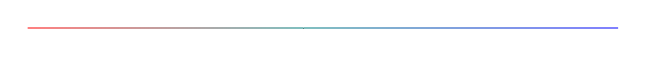
\begin{tikzpicture}
	\fill [left color=red!50, right color=teal!50] (0,0) rectangle (3.5,.01);
	\fill [left color=teal!50, right color=blue!50] (3.5,0) rectangle (7.5,.01);
	\end{tikzpicture}
\vspace{0.5cm}


%%%%%%%%%%%%%%%%%%%%%%%%%%%%%%%%%%%. \begin{ ------>. 
detsacado;  cuadro-naranja;  cuadro-gris;  miejercicio (solución extensa);  mipropuesto (solución corta y fuera del cuadro)

%%%%%%%%%%%%%%%%%%%%%%%%%%%%%%%%%%%. CURIOSIDAD
\vspace{1cm}
\color{ForestGreen!80}
\rule{250pt}{0.2pt}
Texto
\vspace{-8mm}
\begin{flushright}
\rule{250pt}{0.2pt}		
\end{flushright}	
\color{black}
\end{comment}